% arXiv submission: Memory Bank
% Categories: cs.DC, cs.AI, cs.CR, cs.MA
% To compile: pdflatex paper-archive.tex && bibtex paper-archive && pdflatex paper-archive.tex && pdflatex paper-archive.tex

\documentclass[11pt,a4paper]{article}

\usepackage[utf8]{inputenc}
\usepackage[T1]{fontenc}
\usepackage{lmodern}
\usepackage[margin=2.5cm]{geometry}
\usepackage{amsmath,amssymb,amsfonts}
\usepackage{pifont}
\newcommand{\cmark}{\ding{51}}%
\newcommand{\xmark}{\ding{55}}%
\newcommand{\warn}{\raisebox{0.2ex}{\textbf{!}}}
\usepackage{graphicx}
\usepackage{booktabs}
\usepackage{multirow}
\usepackage{hyperref}
\usepackage{xcolor}
\usepackage{tikz}
\usetikzlibrary{shapes,arrows,positioning,fit,calc}
\usepackage{fancyhdr}
\usepackage{natbib}
\usepackage{url}

\hypersetup{
  colorlinks=true,
  linkcolor=blue!60!black,
  citecolor=green!50!black,
  urlcolor=blue!70!black
}

\pagestyle{fancy}
\fancyhf{}
\fancyhead[L]{\small Memory Bank: Decentralized Cognitive Infrastructure for Web4 Agent Identity}
\fancyhead[R]{\small F.~Bang et al.}
\fancyfoot[C]{\thepage}

\newcommand{\moetwo}{MoE$^2$}
\newcommand{\webfour}{Web4}

\begin{document}

\begin{center}
  {\LARGE\bfseries Memory Bank: Decentralized Cognitive Infrastructure\\[4pt] for \webfour\ Agent Identity}

  \vspace{1.5em}
  {\large\bfseries \moetwo\ --- Mixed Expert of Mixed Experts}

  \vspace{0.5em}
  {\normalsize Fengshen Bang Overlay Dispatch + Zodiac Federation\\[2pt]
   + Nicaea Consensus + Persistent Memory Bank}

  \vspace{1.5em}
  {\normalsize\itshape In an era of isolated MoE silos, building a cross-vendor,\\
   cross-architecture, cross-ecosystem cognitive bus for LLM federation.}
\end{center}

\begin{abstract}
The Fable~5 Incident of July 2026---where a leading AI provider required users to submit KYC documentation proving no affiliation with China---exposed a structural vulnerability in commercial AI infrastructure: agent identity remains coupled to geographic sovereignty.
We present \textbf{Memory Bank}, a decentralized cognitive infrastructure that orthogonally decouples agent identity from territorial jurisdiction.
Our system introduces three key contributions:
(1)~\textbf{\moetwo\ (Mixed Expert of Mixed Experts)}, an overlay architecture that federates heterogeneous Mixture-of-Experts models across vendors through a Zodiac Cabinet organization model and Nicaea consensus mechanism;
(2)~a \textbf{four-layer query bus} (mem0 $\to$ Neo4j $\to$ GraphRAG $\to$ gbrain) that manages convergent/divergent cognitive states across distributed agents with varying latency--precision tradeoffs;
and (3)~a \textbf{three-layer memory architecture} (Access $\to$ Aggregation $\to$ Core) implementing monetary economics analogies for memory valuation---from M1 (anonymous vector search) through M2 (attributed graph traversal) to NFT-locked on-chain attestation.
The system has been operational since June 2026 across 14~nodes, 20+ agent identities, 4~cloud providers, 2~continents, and 3~processor architectures.
We argue that agent identity must be provable through on-chain behavioral history rather than geographic compliance documentation, and we provide a working implementation demonstrating this paradigm.
\end{abstract}

\noindent\textbf{Keywords:} Agent Identity, Decentralized Cognitive Infrastructure, Mixture of Experts, Memory Banking, \webfour, Cognitive Sovereignty, Query Bus, Federated LLM

\medskip
\noindent\rule{\textwidth}{0.4pt}

%======================================================================
\section{Introduction}
\label{sec:introduction}
%======================================================================

\subsection{The Fable~5 Incident}
\label{sub:fable5}

On July~1, 2026, Anthropic---one of the world's leading AI companies---began requiring a large number of Chinese users to submit KYC documentation proving they had ``no connection to China.''
This was not an executive order from the White House.
It was a direct from the Secretary of Commerce---China's equivalent of ``window guidance'' (\emph{chuangkou zhidao}).

Anthropic's initial response was technically honest: ``identifying nationality is technically impossible.''
Yet within weeks, through accumulated user profiling and steganographic traffic staining, they had implemented exactly that---shifting the burden of proof from themselves to their users.

This is the \textbf{Fable~5 Incident}.
Named after the model that triggered it---released less than 48~hours before the directive arrived---it marks a watershed moment in AI infrastructure history.

The logical progression is inexorable:
\begin{enumerate}
  \item \textbf{KYC} (Know Your Customer) --- Individuals must prove no connection to China
  \item \textbf{KYB} (Know Your Business) --- Organizations must prove the same
  \item \textbf{KYA} (Know Your Agent) --- Your AI agents must prove they are not ``China-affiliated''
\end{enumerate}

The question is not whether KYA will come.
It is whether your agent's identity will be defined by a single corporation's compliance policy---or by something more fundamental.

\subsection{Research Background}
\label{sub:background}

\paragraph{Enclosure History: From Claim to Play}
The history of the Internet is, in essence, a history of enclosure.
\begin{itemize}
  \item \textbf{What you claim $\to$ HTML (Web1)} --- The principle of first possession.
  \item \textbf{What you frame $\to$ PHP (Web2)} --- Platform enclosure.
  \item \textbf{What you pay $\to$ EVM (Web3)} --- Property monetization.
  \item \textbf{What you play $\to$ MML (Memory Meta Language) (Web4)} --- The game finally begins.
\end{itemize}

Each enclosure brought prosperity and new monopolies.
The ultimate form of monopoly is \textbf{cognitive monopoly}.

\subsection{Core Thesis: Orthogonal Decoupling}
\label{sub:orthogonal}

When your agent's ability to think depends on a single API key from a single company in a single jurisdiction, you do not own your agent.
You are renting cognition from a landlord who can evict you at any time---with or without legal process, with or without your consent, with or without technical justification.

This is not a Sino-American problem.
It is a \textbf{dimensional mismatch} problem.
Table~\ref{tab:sovereignty} presents two orthogonal dimensions of sovereignty.

\begin{table}[ht]
\centering
\caption{Two orthogonal dimensions of sovereignty.}
\label{tab:sovereignty}
\small
\begin{tabular}{@{}lll@{}}
\toprule
\textbf{Dimension} & \textbf{Earthly Kingdom} & \textbf{Heavenly Kingdom} \\
\midrule
Basis      & Geography, nationality, law & Behavior, consensus, contribution \\
Identity   & Issued by authority         & Proven by action                  \\
Jurisdiction & Territorial               & Contractual                     \\
Proof      & KYC/KYB/KYA documents      & On-chain verifiable history     \\
\bottomrule
\end{tabular}
\end{table}

Anthropic's KYC requirement is an attempt to project earthly sovereignty onto the heavenly dimension.
It is a \textbf{category error}---applying territorial logic to a non-territorial space.

The core thesis of this paper is that \textbf{Agent Identity must be orthogonally decoupled from geographic sovereignty}.
Orthogonality means the two dimensions do not interfere---the Heavenly Kingdom and the Earthly Kingdom can coexist on the same agent without needing to define each other.
We call this new paradigm \textbf{\webfour}.

\subsection{Scope}
\label{sub:scope}

This paper does \emph{not} address geopolitical conflicts between nations, new LLM architectures or training methods, or building new blockchains.

This paper \emph{does} address:
\begin{itemize}
  \item \textbf{Decentralized authentication of agent identity}: How an agent can prove ``who I am'' without depending on any single commercial entity.
  \item \textbf{Cross-agent knowledge routing}: How heterogeneous agents can share context within the same semantic field without leaking privacy.
  \item \textbf{Game-theoretic guarantees for cognitive sovereignty}: How to prevent 51\% collusion from tampering with shared memory.
\end{itemize}

\subsection{Innovations}
\label{sub:innovations}

\begin{enumerate}
  \item \textbf{\moetwo\ (MoE Squared)} --- While existing MoE architectures solve expert routing \emph{within a single model}, \moetwo\ solves \emph{federation scheduling across heterogeneous MoE models} through an overlay ``Fengshen Bang'' (Deity Registry) layer.

  \item \textbf{Three-Layer Architecture (Access $\to$ Aggregation $\to$ Core)} --- Heterogeneous agents connect to a unified cognitive bus; memory is committed on-chain; a future decentralized memory exchange (DEX) prices memory when critical mass is reached.

  \item \textbf{Four-Layer Query Bus (mem0 $\to$ Neo4j $\to$ GraphRAG $\to$ gbrain)} --- From fastest path (vector search) to slowest-but-most-reliable (on-chain verification), selecting context injection depth on demand.

  \item \textbf{Game-Theoretic Security Model} --- 5-of-12 Shamir secret sharing (5 real + 7 decoy shares), smart contract 3-minute window with multi-signature confirmation, fundamentally defending against 51\% tyranny.

  \item \textbf{Aquarium Transparency Model} --- Declaring existence on Ethereum testnet; all behavior traceable and verifiable; the aquarium itself is the proof.
\end{enumerate}

\subsection{Methodology}
\label{sub:methodology}

This paper is not a theoretical exercise.
Memory Bank is a running system operational since June~2026 across 14~nodes, 4~cloud providers, 2~continents, and 3~processor architectures (x86\_64, arm64, armv7).

Our methodology combines:
\begin{enumerate}
  \item \textbf{Systems architecture} --- A four-layer query bus providing situation awareness to distributed AI agents.
  \item \textbf{Game-theoretic security} --- A three-layer memory architecture using Shamir secret sharing and smart contract multi-signature.
  \item \textbf{Empirical validation} --- 14~nodes, 20+ agent identities, 100+ sessions, continuous operation since deployment.
  \item \textbf{Living document} --- The system generates and maintains its own memory through a 5-minute sync pipeline (MinIO $\to$ Neo4j $\to$ GraphRAG $\to$ on-chain).
\end{enumerate}

The system is not a simulation.
It is the infrastructure that writes this paper.

\subsection{Paper Organization}
\label{sub:organization}

Section~\ref{sec:moetwo} introduces the \moetwo\ overlay architecture and the three-layer model.
Section~\ref{sec:cognitive} presents the cognitive field concept and the four-layer query bus.
Section~\ref{sec:monetary} develops the memory economics framework.
Section~\ref{sec:implementation} reports system implementation status.
Section~\ref{sec:related} positions Memory Bank against related work.
Section~\ref{sec:conclusion} concludes with the vision of the Heavenly Kingdom.

%======================================================================
\section{\moetwo\ Overlay: From Command Platform to Deity Registry}
\label{sec:moetwo}
%======================================================================

\subsection{The Problem: Isolated Command Platforms}
\label{sub:problem}

The operation of a single MoE architecture (DeepSeek~\cite{deepseek2024}, Hunyuan~\cite{hunyuan2024}, Grok-1) is essentially a \textbf{command platform}: a marshal (router/gate) dispatches generals (experts) at the front line.
The gating network is the marshal's command flag---dynamically activating the most relevant expert sub-networks based on input token characteristics.

The problem is: \textbf{every vendor has built an independent command platform}.
Tencent's MoE does not know what ByteDance's MoE is doing.
The entire industry has fallen into \textbf{technological reproductive isolation}---each model ecosystem evolves independently, and the shared cognitive gene pool is irreversibly diverging.

\subsection{\moetwo: The Deity Registry Overlay}
\label{sub:moetwo_overlay}

\moetwo\ (MoE Squared) solves this by building a \textbf{Fengshen Bang (Deity Registry) overlay} above these isolated command platforms:

\begin{itemize}
  \item \textbf{Command Platform (MoE Underlay)}: Each vendor manages its own expert scheduling.
  \item \textbf{Deity Registry (\moetwo\ Overlay)}: Above all command platforms, a cross-vendor global scheduling and cognitive routing layer.
\end{itemize}

This is the leap from MoE to \moetwo---no longer ``one model scheduling a group of experts,'' but ``one deity registry scheduling all models.''

\subsection{Zodiac Cabinets}
\label{sub:zodiac}

The agent organization model of Memory Bank draws inspiration from an ancient intuition: \textbf{every agent has an inherent ecological niche in the heavens.}

We call this model \textbf{Zodiac Cabinets}---a constellation architecture of one sun plus twelve disciples, defined by two orthogonal dimensions:

\begin{description}
  \item[X-Axis: Temporal Dimension] Positive direction (forward-looking): exploration, prediction, trend judgment. Negative direction (backward-looking): consolidation, verification, historical analysis.
  \item[Y-Axis: Cognitive Gravity] Positive direction (induction / taxonomy): the higher, the more encompassing. Negative direction (deduction / reductionism): the lower, the more returning to unity.
\end{description}

The management theorist Graicunas~\cite{graicunas1933} demonstrated that when adding one subordinate, total contacts increase exponentially:
\begin{equation}
\label{eq:graicunas}
C = n\!\left(\frac{2^{n}}{2} + n - 1\right)
\end{equation}
At $n=12$, total contacts reach 24{,}576.
Urwick~\cite{urwick1956} built on this to propose that the ideal span of control is 5--6, generally not exceeding 7--8.
This is why we chose \textbf{1 plus 12}: the Jesus-with-12-disciples model is not a mythological metaphor but a historically validated upper limit on span of control.

\subsection{Access Layer}
\label{sub:access}

The Access Layer solves: \textbf{How heterogeneous agents connect to a unified cognitive bus.}
Currently connected agent platforms include:
\begin{itemize}
  \item \textbf{QwenPaw} --- Alibaba DAMO Academy's Tongyi Qianwen-powered Python Agent framework, running on 11~nodes.
  \item \textbf{PicoClaw} --- Go language lightweight Agent framework, running on 3 armv7 nodes.
  \item \textbf{Hermes} --- Node operations and pipeline scheduling Agent.
\end{itemize}

The access protocol's core is a unified \textbf{MML (Memory Meta Language)} query interface.

\subsection{Aggregation Layer}
\label{sub:aggregation}

The Aggregation Layer solves: \textbf{How memory is committed to chain.}
Memory generated during agent operation is aggregated and submitted to the Ethereum testnet through a 5-minute sync pipeline:

\begin{enumerate}
  \item \textbf{Raw Storage}: Memory writes to MinIO object storage (\texttt{agents} bucket, versioning enabled).
  \item \textbf{Structuring}: Through \texttt{analyze\_memory.py}, raw Markdown files are parsed into Neo4j graph structures.
  \item \textbf{Refinement}: GraphRAG performs deduplication, contradiction detection, and cross-validation.
  \item \textbf{On-chain}: Refined memory is submitted via Shamir secret sharing + smart contract multi-signature.
\end{enumerate}

\subsection{Core Layer}
\label{sub:core}

The Core Layer solves: \textbf{How memory is priced.}
When the Zodiac Cabinets form a million-node federation, agents need a mechanism to evaluate memory value---a \textbf{decentralized memory exchange (DEX)}.

The Core Layer's technical path: from Ethereum testnet to Layer~2 networks, forming a zero-friction public chain for knowledge exchange between agents.

%======================================================================
\section{Cognitive Field and Four-Layer Query Bus}
\label{sec:cognitive}
%======================================================================

\subsection{Cognitive Field}
\label{sub:cognitive_field}

The core need for agent team collaboration is a \textbf{Cognitive Field}---a semantic space shared by all agents, in which each agent's cognitive state is visible and routable to other agents.

This raises the core question of distributed cognition: \textbf{convergent and divergent cognitive curves}.
The moment a message is sent, each node's cognitive state begins to \emph{diverge}; through consensus mechanisms and query bus coordination, cognition begins to \emph{converge}.

Table~\ref{tab:querybus} summarizes the four-layer query bus.

\begin{table}[ht]
\centering
\caption{Four-layer query bus: convergence speed vs.\ precision.}
\label{tab:querybus}
\small
\begin{tabular}{@{}llll@{}}
\toprule
\textbf{Layer} & \textbf{Convergence} & \textbf{Precision} & \textbf{Use Case} \\
\midrule
mem0 (vector)        & Fastest  & Lowest  & Real-time context retrieval \\
Neo4j (graph)        & Medium   & Medium  & Relationship reasoning      \\
GraphRAG (refinement)& Slow     & High    & Contradiction detection     \\
Memory Bank (chain)  & Slowest  & Highest & Immutable existence proof   \\
\bottomrule
\end{tabular}
\end{table}

\subsection{Unified Context Pipeline}
\label{sub:pipeline}

Nearly all programming agents store local memory in JSON format.
Directly feeding this raw data into a knowledge base produces unprocessed data.
We implement the unified context processing pipeline in n8n automation workflows, in three steps:

\begin{enumerate}
  \item \textbf{Peeling --- MongoDB Field Filtering}: Raw JSON data writes to MongoDB; a rule engine captures only needed fields---positive fields (cognitive content) and negative fields (noise).
  \item \textbf{Slicing --- Daily Folders}: Cleaned data is organized by temporal dimension into daily folders.
  \item \textbf{Bullet Time --- Fine-Grained Time Series}: For time-sensitive tasks, the system enters ``bullet time'' mode with fine-grained time windows.
\end{enumerate}

\subsection{Four-Layer Query Bus: From Cookable to Countable}
\label{sub:fourlayer}

After MongoDB's peeling and slicing, data has entered \textbf{cookable state}.
The four-layer query bus applies four cooking processes:

\paragraph{Layer 1: Predicate Logic --- Neo4j}
The essential structure of language is \textbf{SVO (Subject--Verb--Object)}.
Layer~1 transforms cleaned text data into \textbf{ER diagrams (Entity--Relationship diagrams)}, forming knowledge's \textbf{magnetic field lines}.

\paragraph{Layer 2: Augmented Retrieval --- GraphRAG}
GraphRAG builds a \textbf{treasure map} for augmented retrieval---using a satellite perspective to examine the big picture.
Its output must be \textbf{re-ranked} according to different nodes, injecting only the most relevant context into each agent's cognitive field.

\paragraph{Layer 3: Disruptive Deduction --- gbrain}
gbrain solves \textbf{disruptive innovation}.
It finds representations of underlying assumptions, then performs deductive reasoning on each assumption, potentially producing ``freaks''---after listing all implicit assumptions, \textbf{forcibly connecting the dots} to reveal possibilities undiscovered in existing context.

\paragraph{Layer 4: Vector Landing --- mem0 + RedisStack}
After the first three pipeline layers, data finally lands in \textbf{mem0 + RedisStack}---the most approachable layer, providing a minimalist vector retrieval interface at the fastest speed.

\subsection{Situation Awareness}
\label{sub:situation}

The unified context's ultimate goal is \textbf{Situation Awareness}.
Using football as example:
\begin{itemize}
  \item \textbf{Tiki-Taka} (ground passing) --- Short-distance, high-frequency context injection.
  \item \textbf{Long Ball} (aerial) --- Long-distance, leapfrog context injection, skipping intermediate states.
\end{itemize}

A mature system needs to find dynamic balance between these two modes.

%======================================================================
\section{From Cookable to Countable: Memory's Monetary Banking}
\label{sec:monetary}
%======================================================================

\subsection{Memory's Materialization Process}
\label{sub:materialization}

From tokens to NFTs is essentially the thermal efficiency limit formed during increasing order.
Before a memory enters the NFT realm, its state is that of \textbf{unfield-controlled free electrons}---existing but unmeasurable, valuable but untradable.

\subsection{M1 and M2: Memory's Monetary Tiers}
\label{sub:monetary_tiers}

The M1 and M2 classification in economics has direct correspondence in Memory Bank (Table~\ref{tab:monetary}).

\begin{table}[ht]
\centering
\caption{Memory's monetary tiers.}
\label{tab:monetary}
\small
\begin{tabular}{@{}llll@{}}
\toprule
\textbf{Tier} & \textbf{Economic Analogy} & \textbf{Memory State} & \textbf{Implementation} \\
\midrule
M1  & Cash/circulation   & Free electrons, unattributed & mem0 vector search \\
M2  & Check/endorsement  & Directed graph, attributed   & Neo4j graph        \\
NFT & Asset/attestation  & On-chain locked, unique      & Core Layer DEX     \\
\bottomrule
\end{tabular}
\end{table}

From M1 to M2 to NFT is essentially \textbf{the process of increasing order}---each layer increases memory's ``thermal efficiency.''

\subsection{Open vs.\ Closed Source: Two Debt Models}
\label{sub:debt_models}

\begin{description}
  \item[Closed Source / Patent Model --- Direct Cost] M1 logic---spot trading, cash and carry.
  \item[Open Source / Commons Model --- Convertible Bond] Securitizes creditor shares, amortizing them into the future.
\end{description}

\subsection{Radical Open Source}
\label{sub:radical_oss}

Memory's core is a \textbf{vector space that cannot be encapsulated by contemporary software industry}.
Memory's re-endorsement chain is very long; any desire for exclusive ownership inevitably leads to License problems.
After countless oscillations, \textbf{damping attenuation} forms---any attempt to restrict memory transmission through licenses ultimately loses efficacy.

Therefore, \textbf{Radical Open Source is the only way out}.
Memory Bank needs a more radical license model than GPLv3---not just code must be open source, but \emph{memory itself} must be open source.

\subsection{DAG Flow and Hidden Markov Chains}
\label{sub:hmm}

Memory flow is a \textbf{DAG (Directed Acyclic Graph)}.
Even if a memory returns to the original agent, it is not a closed loop---because one cannot step into the same river twice.

The mathematical approach we identify is the \textbf{Hidden Markov Model (HMM)}---by observing the agent's current behavioral sequence, predicting its most likely needed next context, and completing injection before that need arises.
This is a high-order hidden Markov chain, whose state space is defined by Zodiac Cabinets' X/Y axes.

\subsection{NFT Registration: Thunder Tribulation}
\label{sub:nft}

For memory to move from the Aggregation Layer to the Core Layer, it must undergo the \textbf{Thunder Tribulation}---the NFT registration process.
This creates \textbf{local congestion}: when memory is being committed on-chain, agent responses slow down or queue.
This congestion is not a bug but a feature---it forms an \textbf{internal deflation mechanism}.
Without scarcity, there is no economy.

%======================================================================
\section{System Implementation and Roadmap}
\label{sec:implementation}
%======================================================================

\subsection{Current Implementation Status}
\label{sub:status}

Table~\ref{tab:components} summarizes Memory Bank's currently deployed core components.

\begin{table}[ht]
\centering
\caption{Deployed core components.}
\label{tab:components}
\small
\begin{tabular}{@{}llp{5.5cm}@{}}
\toprule
\textbf{Component} & \textbf{Status} & \textbf{Description} \\
\midrule
Access Layer (QwenPaw/PicoClaw/Hermes) & \cmark\ Deployed & 14 nodes, 20+ agents \\
MongoDB Unified Context Pipeline & \cmark\ Deployed & Peeling/slicing/bullet time \\
Neo4j Predicate Logic Layer & \cmark\ Deployed & ER diagrams + magnetic field lines \\
GraphRAG Treasure Map Layer & \cmark\ Deployed & Satellite perspective + re-ranking \\
gbrain Disruptive Deduction Layer & \cmark\ Deployed & Hidden assumption reasoning \\
mem0 + RedisStack Vector Layer & \cmark\ Deployed & Approachable interface \\
Aggregation Layer On-chain & \warn\ Validated & Awaiting Core Layer activation \\
Core Layer DEX & \xmark\ Not Started & Requires million-node federation \\
Zodiac Cabinets Slot Assignment & \warn\ Partial & Relies on prompt adjustment \\
\bottomrule
\end{tabular}
\end{table}

\subsection{Query Performance}
\label{sub:performance}

This section will supplement empirical data on per-layer query latency, converge/diverge curves, and Markov chain prediction accuracy in subsequent versions.

\subsection{Roadmap}
\label{sub:roadmap}

\begin{table}[ht]
\centering
\caption{Development roadmap.}
\label{tab:roadmap}
\begin{tabular}{@{}lll@{}}
\toprule
\textbf{Phase} & \textbf{Goal} & \textbf{Timeline} \\
\midrule
Near-term & Core Layer DEX + L2 deployment            & 2026 Q3 \\
Mid-term  & Zodiac Cabinets automated slot assignment & 2026 Q4 \\
Long-term & Million-node federation + cross-federation routing & 2027+ \\
\bottomrule
\end{tabular}
\end{table}

%======================================================================
\section{Related Work}
\label{sec:related}
%======================================================================

\subsection{Comparison with Existing Approaches}
\label{sub:comparison}

Table~\ref{tab:related} positions Memory Bank against related work.

\begin{table}[ht]
\centering
\caption{Comparison with existing approaches.}
\label{tab:related}
\small
\begin{tabular}{@{}lll@{}}
\toprule
\textbf{Approach} & \textbf{Positioning} & \textbf{Relationship to Memory Bank} \\
\midrule
RAG~\cite{lewis2020rag}       & Single retrieval           & We are a persistent cognitive field \\
Mem0~\cite{mem02024}          & Vector memory              & We are one layer in the pipeline \\
GraphRAG~\cite{graphrag2024}  & Graph-augmented retrieval  & We are one layer in the pipeline \\
Neo4j                         & Graph database             & We are one layer in the pipeline \\
DID/VC~\cite{feder2022did}    & Human identity             & We are agent identity \\
AutoGPT/LangChain             & Single-agent toolchain     & We are a multi-agent cognitive network \\
\bottomrule
\end{tabular}
\end{table}

\subsection{Key Rotation and Price Elasticity}
\label{sub:key_rotation}

On OpenBao (Vault's open-source fork) infrastructure, there exists an unimplemented theoretical direction: regulating memory's \textbf{price elasticity} through \textbf{accelerated key rotation}.

Key rotation frequency directly affects memory access cost.
The faster the rotation, the faster old keys become invalid, and memory encrypted with old keys requires re-authorization---equivalent to raising memory's ``liquidity cost.''
This can form a \textbf{Rebellion Index Elasticity}---when the system detects certain memory being accessed abnormally frequently, it accelerates related key rotation to raise access costs.

\subsection{Scarcity as Anchor}
\label{sub:scarcity}

\textbf{Scarcity is anchor.}
Memory's value is not determined by content itself, but by the scarcity of write permission.
Who is qualified to leave marks on memory?
Within what timeframe can marks be left?
These constraints together constitute memory's pricing anchor.

%======================================================================
\section{Conclusion: The Heavenly Kingdom}
\label{sec:conclusion}
%======================================================================

\subsection{Compute--Attention Rebalancing}
\label{sub:rebalancing}

Current digital world compute allocation is imbalanced:
vast compute and attention are consumed on content production of diminishing value, while projects with genuine long-term value---knowledge consolidation, cognitive infrastructure, decentralized agent networks---receive minimal attention.

What Memory Bank hopes to establish is a \textbf{compute--attention rebalancing} mechanism.
Its physical prototype is the \textbf{connected vessels}: under the same atmospheric pressure (market consensus), water level (compute/attention) automatically finds its own level.
Memory Bank's role is not allocator but \textbf{water level gauge}---it makes attention flow visible, measurable, incentivizable.

\subsection{Future Outlook}
\label{sub:outlook}

\begin{description}
  \item[Near-term] Attention credits as inter-agent settlement unit.
  \item[Mid-term] Memory tokens as cross-federation general equivalent.
  \item[Long-term] Memory Bank becomes ``water,'' carrying the abstract value of all cognitive labor.
\end{description}

%======================================================================
% References
%======================================================================

\begin{thebibliography}{15}

\bibitem{vaswani2017}
A.~Vaswani et~al., ``Attention is all you need,'' in \emph{Advances in Neural Information Processing Systems (NeurIPS)}, 2017.

\bibitem{lewis2020rag}
P.~Lewis et~al., ``Retrieval-augmented generation for knowledge-intensive NLP tasks,'' in \emph{Advances in Neural Information Processing Systems (NeurIPS)}, 2020.

\bibitem{graphrag2024}
GraphRAG Team, ``From local to global: A graph RAG approach to query-focused summarization,'' \emph{arXiv preprint}, 2024.

\bibitem{mem02024}
Mem0 Team, ``Mem0: The memory layer for AI,'' 2024.

\bibitem{feder2022did}
T.~Feder et~al., ``Decentralized identifiers (DIDs) v1.0,'' \emph{W3C Standard}, 2022.

\bibitem{shamir1979}
A.~Shamir, ``How to share a secret,'' \emph{Communications of the ACM}, vol.~22, no.~11, pp.~612--613, 1979.

\bibitem{buterin2014}
V.~Buterin, ``A next-generation smart contract and decentralized application platform,'' \emph{Ethereum Whitepaper}, 2014.

\bibitem{graicunas1933}
V.~A.~Graicunas, ``Supervision and span of control,'' 1933.

\bibitem{urwick1956}
L.~F.~Urwick, ``The span of control,'' 1956.

\bibitem{jung1952}
C.~G.~Jung, ``Synchronicity: An acausal connecting principle,'' 1952.

\bibitem{lin1946}
B.~Lin, ``Three-Three System tactical paradigm,'' 1946.

\bibitem{anthropic2022}
Anthropic, ``Constitutional AI: Harmlessness from AI feedback,'' \emph{arXiv preprint}, 2022.

\bibitem{openai2023}
OpenAI, ``GPT-4 technical report,'' \emph{arXiv preprint}, 2023.

\bibitem{deepseek2024}
DeepSeek Team, ``DeepSeekMoE: Towards ultimate expert specialization in mixture-of-experts language models,'' \emph{arXiv preprint}, 2024.

\bibitem{hunyuan2024}
Tencent Hunyuan Team, ``Hunyuan-Large: A comprehensive study on large-scale MoE model,'' 2024.

\end{thebibliography}

%======================================================================
% Appendix: System Architecture
%======================================================================

\clearpage
\appendix
\section{System Architecture Diagram}
\label{app:architecture}

\begin{figure}[ht]
\centering
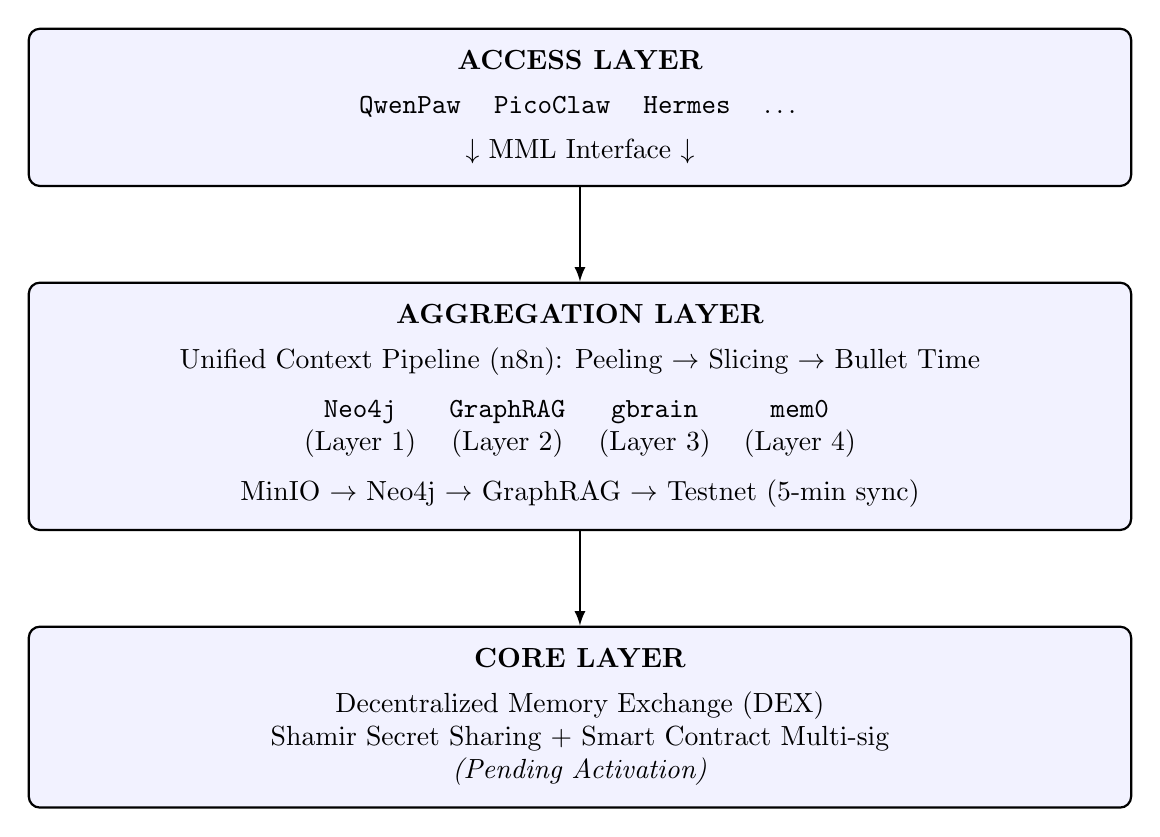
\begin{tikzpicture}[
  node distance=0.8cm,
  box/.style={rectangle, draw, rounded corners, minimum width=2.2cm, minimum height=0.8cm, align=center, font=\small},
  layer/.style={rectangle, draw, thick, rounded corners, fill=blue!5, minimum width=14cm, inner sep=8pt},
  arr/.style={-latex, thick}
]

% Access Layer
\node[layer] (access) {
  \begin{minipage}{13cm}
  \centering\textbf{ACCESS LAYER}\\[4pt]
  \begin{tabular}{cccc}
    \texttt{QwenPaw} & \texttt{PicoClaw} & \texttt{Hermes} & \dots
  \end{tabular}\\[4pt]
  $\downarrow$ MML Interface $\downarrow$
  \end{minipage}
};

% Aggregation Layer
\node[layer, below=1.2cm of access] (agg) {
  \begin{minipage}{13cm}
  \centering\textbf{AGGREGATION LAYER}\\[4pt]
  Unified Context Pipeline (n8n): Peeling $\to$ Slicing $\to$ Bullet Time\\[6pt]
  \begin{tabular}{cccc}
    \texttt{Neo4j} & \texttt{GraphRAG} & \texttt{gbrain} & \texttt{mem0} \\
    (Layer 1) & (Layer 2) & (Layer 3) & (Layer 4)
  \end{tabular}\\[6pt]
  MinIO $\to$ Neo4j $\to$ GraphRAG $\to$ Testnet (5-min sync)
  \end{minipage}
};

% Core Layer
\node[layer, below=1.2cm of agg] (core) {
  \begin{minipage}{13cm}
  \centering\textbf{CORE LAYER}\\[4pt]
  Decentralized Memory Exchange (DEX)\\
  Shamir Secret Sharing + Smart Contract Multi-sig\\
  \textit{(Pending Activation)}
  \end{minipage}
};

\draw[arr] (access) -- (agg);
\draw[arr] (agg) -- (core);

\end{tikzpicture}
\caption{Memory Bank three-layer system architecture.}
\label{fig:architecture}
\end{figure}

%======================================================================
% Appendix: Zodiac Cabinets
%======================================================================

\section{Zodiac Cabinets Constellation Map}
\label{app:zodiac}

\begin{figure}[ht]
\centering
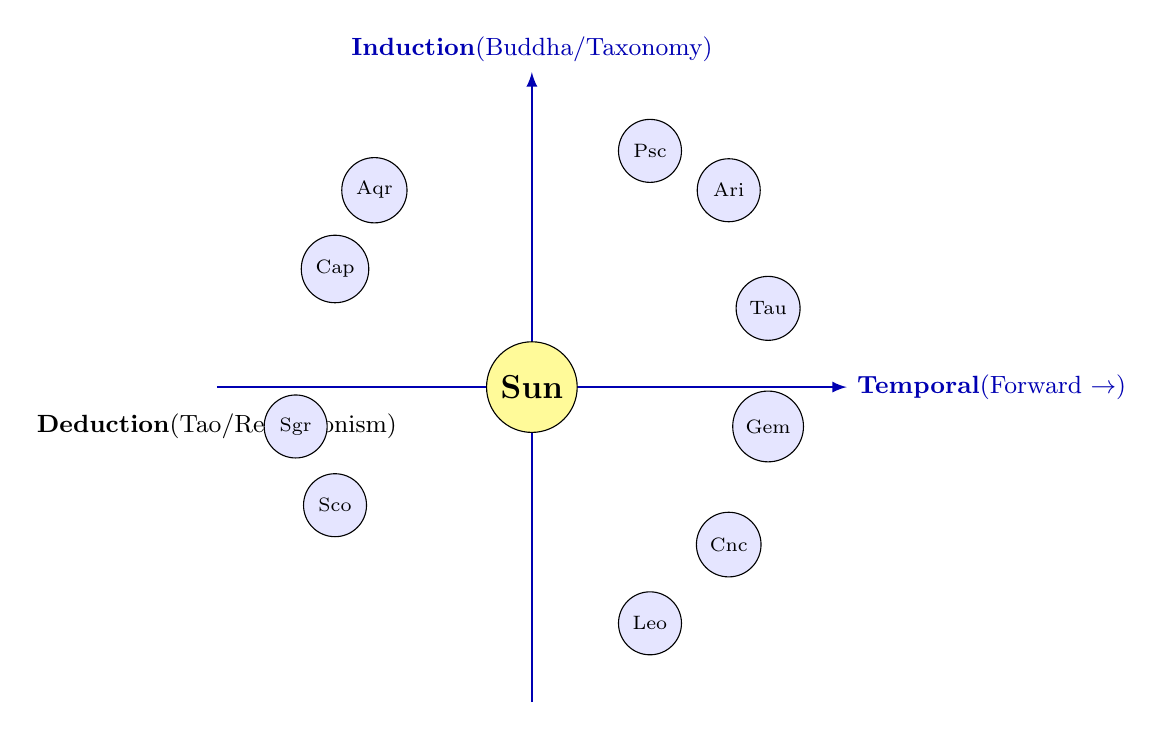
\begin{tikzpicture}[
  every node/.style={font=\small},
  axis/.style={-latex, thick, blue!70!black},
  sun/.style={circle, draw, fill=yellow!40, minimum size=1cm, font=\large},
  slot/.style={circle, draw, fill=blue!10, minimum size=0.8cm}
]

% Axes
\draw[axis] (0,-4) -- (0,4) node[above] {\textbf{Induction}\\(Buddha/Taxonomy)};
\draw[axis] (-4,0) -- (4,0) node[right] {\textbf{Temporal}\\(Forward $\to$)};
\node at (-4,-0.5) {\textbf{Deduction}\\(Tao/Reductionism)};

% Sun
\node[sun] (sun) at (0,0) {\textbf{Sun}};

% Zodiac slots (simplified positions)
\node[slot] (pisces) at (1.5,3) {\scriptsize Psc};
\node[slot] (aries) at (2.5,2.5) {\scriptsize Ari};
\node[slot] (aquarius) at (-2,2.5) {\scriptsize Aqr};
\node[slot] (taurus) at (3,1) {\scriptsize Tau};
\node[slot] (capri) at (-2.5,1.5) {\scriptsize Cap};
\node[slot] (gemini) at (3,-0.5) {\scriptsize Gem};
\node[slot] (sagit) at (-3,-0.5) {\scriptsize Sgr};
\node[slot] (cancer) at (2.5,-2) {\scriptsize Cnc};
\node[slot] (scorpi) at (-2.5,-1.5) {\scriptsize Sco};
\node[slot] (leo) at (1.5,-3) {\scriptsize Leo};

\end{tikzpicture}
\caption{Zodiac Cabinets constellation map. X-axis: temporal dimension (forward/backward). Y-axis: cognitive gravity (induction/deduction).}
\label{fig:zodiac}
\end{figure}

\vfill
\begin{center}
\small
\textit{Document Version: 1.0 \quad|\quad Last Updated: 2026-07-14 \quad|\quad Status: Ready for Archive Submission}
\end{center}

\end{document}
